\chapter{动量}\label{chp:momentum}
\section{冲量和动量}
一辆汽车,受到不同的牵引力时,从开动到获得一定的速度,需要的时间不同。
牵引力大,需要的时间短,牵引力小,需要的时间长。

现在我们来定量地研究一下这类问题。
一个质量为 $m$ 的物体,原来静止,在力 $F$ 的作用下,经过时间 $t$,将获得多大的速度?
这个问题利用牛顿运动定律很容易解决。
物体在力 $F$ 的作用下得到加速度 $a=F/m$,经过时间 $t$ 后,在 $t$ 秒末的速度 $v=at=Ft/m$。由此得到
\[Ft=mv.\]

可见,要使原来静止的某物体获得某一速度,可以有不同的方法,既可以用较大的力作用较短的时间,也可以用较小的力作用较长的时间;只要力和力的作用时间的乘积 $Ft$ 相同,这个物体总得到相同的速度。
这就是说,对一定质量的物体,力所产生的改变物体速度的效果,是由 $Ft$ 这个物理量决定的。
在物理学中,\emph{力和力的作用时间的乘积 $Ft$ 叫做力的}\Concept{冲量}。

冲量是个矢量,它的方向由力的方向决定。
如果在作用时间内力的方向不变,冲量的方向就是力的方向。
冲量的单位由力和时间的单位决定,在国际单位制里,冲量的单位是牛\,$\cdot$\,秒{\unit{N.s}}。

从上式还可以看出,原来静止的不同的物体,在相同冲量的作用下,它们得到的速度不同,质量大的物体得到的速度小,质量小的物体得到的速度大,但是它们的质量和速度的乘积$mv$ 却是相同的,都等于它们受到的冲量。
在物理学中,\emph{质量和速度的乘积 $mv$ 叫做}\Concept{动量}。

动量常用符号 $p$ 表示,动量也是矢量,它的方向就是速度的方向。
在国际单位制中,动量的单位是千克\,$cdot$\,米/秒(\unit{kg.m/s})。
动量的单位跟冲量的单位实际上是相同的,由于 $\qty{1}{N}=\qty{1}{kg.m/s^2}$,所以 $\qty{1}{N.s}=\qty{1}{kg.m/s}$。

在物理学里,动量是个很重要的量,经常要用到。
动量和速度虽然彼此有关,但含义是不同的。
速度是运动学上的一个物理量,它描述物体运动的快慢和方向。
只有速度的概念,并不能说明使物体得到这个速度或使以这个速度运动的物体停止下来,需要多大的冲量。
为了说明这类问题,就要引入动量的概念,动量是动力学上的一个物理量。
例如,要使以相同的速度运动的铅球和乒乓球停止下来,铅球需要的冲量大,就是因为铅球的质量大,动量也大的缘故。

动量既然是矢量,它的加法要服从矢量运算规则,即按照平行四边形法则来进行。
如果物体的运动在同一条直线上,即动量矢量在同一条直线上,那么,在选定一个正方向之后,动量矢量的运算就简化成代数运算了。

\begin{example}
一个质量是 \qty{0.1}{kg} 的钢球以 \qty{6.0}{m/s} 的速度向右运动,碰到一个坚硬的障碍物后弹回,沿同一直线以 \qty{6.0}{m/s} 的速度向左运动,碰撞前后钢球的动量有没有变化?变化了多少?
\end{example}

\begin{solution}
取向右的方向为正方向,钢球碰到障碍物前,它的速度 $v=\qty{6}{m/s}$,这时钢球的动量
\[p=mv=\qty{6.0}{kg.m/s},\]
碰到障碍物后,钢球的速度 $v'=\qty{-6.0}{m/s}$,这时钢球的动量
\[p'=mv'=\qty{-6.0}{kg.m/s}.\]
可见钢球的动量发生了变化,钢球动量的变化等于变化后的动量减去变化前的动量,所以钢球动量的变化为
\[p'-p=\qty{-12}{kg.m/s}.\]
\end{solution}

\begin{Practice}
\begin{question}
  \item 用 \qty{4}{N} 的力推动一个物体,力的作用时间是 \qty{0.5}{s},力的冲量是多少?
  \item 使质量为 \qty{4}{t} 的汽车,从静止达到 \qty{20}{km/h} 的速度,需要多大的冲量?
  \item 质量是 \qty{25}{kg} 以 \qty{0.5}{m/s} 的速度步行的小孩和质量是 \qty{0.02}{kg} 以 \qty{800}{m/s} 的速度飞行的子弹,哪个动量大?
  \item 质量为 \qty{8}{g} 的玻璃弹球以 \qty{3}{m/s} 的速度向左运动,碰到一个物体后弹回,以 \qty{2}{m/s} 的速度沿同一直线向右运动,弹球的动量改变了多少?
  \item 以相同的速度分别向竖直和水平方向抛出两个质量相等的物体,抛出时两个物体的动能是否相等?动量是否相等?
\end{question}
\end{Practice}

\section{动量定理}
现在我们进一步证明,如果物体原来就是运动的,已经具有一定的动量,在合外力的作用下,经过一段时间,速度要发生变化,因而动量也发生变化,这时,物体所受的合外力的冲量等于它的动量的变化。

设一个质量为 $m$ 的物体,原来的速度是 $v$,在恒定的外力作用下得到加速度 $a=F/m$,经过时间 $t$ 速度变成 $v'$,速度的变化就是 $v'-v=at$。
由此可得
\[Ft=mat=mv'-mv.\]
由于变化前的动量 $p=mv$,变化后的动量 $p'=mv'$,所以上式可以改写成
\[Ft=p'-p.\]
这就是说,\emph{物体所受合外力的冲量等于它的动量的变化}。
这个结论叫做\Concept{动量定理}。

从动量定理可以知道,如果一个物体的动量的变化是一定的,那么,它受力作用的时间越短,这个力就越大,力作用的时间越长,这个力就越小。
利用这个道理可以解释为什么茶杯掉在石头上立即摔碎,掉在软的东西上不易摔碎。
茶杯碰到物体以前,以一定的速度运动着,动量为 $mv$,碰到物体后,停止运动,动量变为 0。在这个过程中,茶杯动量的变化是 $-mv$,这个值等于茶杯受到的作用力的冲量。
掉在石头上,茶杯从运动到停止经历的时间短,受到的石头的作用力大,因此碎掉。
掉在软的东西上,茶杯从运动到停止经历的时间长,受到的作用力小,因此不易破碎。
搬运玻璃等易碎物品时,在木箱里放些纸屑、刨花等物,可以减少搬运中的损坏,也是这个道理。

动量定理不但适用于恒定的外力,而且适用于随时间而变化的变力。
在后一种情况下,动量定理中的力 $F$ 应理解为变力在作用时间内的平均值。

\begin{example}
用 \qty{5.0}{kg} 的铁锤把道钉打进铁路的枕木里去,打击时铁锤的速度是 \qty{5.0}{m/s}。如果打击的作用时间是 \qty{0.01}{s},求打击时的平均作用力,不计铁锤的重量。
\end{example}

\medskip\noindent
\begin{minipage}{0.76\linewidth}
\begin{solution}
打击时,铁锤和道钉受到的力如\cref{fig:8-1} 所示。
不计铁锤的重量,只考虑铁锤受到的道钉的作用力 $N$。
铁锤在这个力的作用下,在 $t=\qty{0.01}{s}$ 内,速度由 $v=\qty{-5.0}{m/s}$,变为 $v'=0$,这里取竖直向上的方向为正方向。
应用动量定理就可以求出平均作用力:
\[\begin{split}
    N&=\frac{p'-p}{t}=\frac{mv'-mv}{t}\\
    &=\frac{0-5.0\times (-5.0)}{0.01}\,\unit{N}\\
    &=\qty{2.5e3}{N}.
\end{split}\]
道钉所受的打击力 $F$,与铁锤所受的力大小相等,方向相反,也是 \qty{2.5e3}{N}。
\end{solution}
\end{minipage}\hfill
\begin{minipage}{0.2\linewidth}
  \begin{figurehere}
    \includegraphics{8-1.pdf}
    \caption{}\label{fig:8-1}
  \end{figurehere}
\end{minipage}

\medskip
讨论:上述计算中没有考虑铁锤的重量,如果把铁锤的重量也考虑在内,那么,这时道钉所受的打击力是上面算出的打击力加上铁锤的重量。
而铁锤的重量
\[G=5.0\times \qty{9.8}{N}=\qty{49}{N}, \]
与上面算出的打击力 \qty{2.5e3}{N} 相比,铁锤的重量约为后者的 2\%,可见在计算打击过程中的平均作用力时,不考虑铁锤的重量是可以的。

\begin{Practice}
\begin{question}
  \item \qty{10}{kg} 的物体以 \qty{10}{m/s} 的速度作直线运动,在受到一个恒力作用 \qty{4.0}{s} 后,速度变为反向 \qty{2.0}{m/s}。求:
  \begin{enumerate}
    \item 物体在受力前和受力后的动量;
    \item 物体受到的冲量;
    \item 力的大小和方向。
  \end{enumerate}
  \item 列车的质量是 \qty{2.5e6}{kg},受到的牵引力是 \qty{4.0e5}{N},它的速度由 \qty{10}{m/s} 增加到 \qty{24}{m/s} 需要用多少时间?
  \item 一个质量是 \qty{65}{kg} 的人从墙上跳下,以 \qty{7}{m/s} 的速度着地,与地面接触后 \qty{0.01}{s} 停了下来,地面对他的作用力是多大?如果他着地时弯曲双腿,用了 \qty{1}{s} 才停下来,地面对他的作用力又是多大?
  \item 跳远时,为什么跳在砂坑里比跳在混凝土路面上安全?钉钉子时,为什么要用铁锤而不用橡皮锤?
  \item 质量为 \qty{4}{kg} 的铅球和质量为 \qty{0.1}{kg} 的皮球以相同的速度运动着,要使它们在相同的时间内停下来,作用在铅球上的力和作用在皮球上的力哪个大?为什么?
\end{question}
\end{Practice}

\section{相互作用的物体的动量变化}\label{sec:momentum_change}
我们经常可以看到,物体在相互作用的时候,它们的动量会发生变化。
例如,在滑冰场上原来静止的两个人,无论谁推谁一下,两人就会向相反的方向运动起来(\cref{fig:8-2}),他们的动量都发生了变化。
又例如,在射击的时候,子弹向前飞出,同时枪身后退,子弹和枪身的动量也都发生了变化。
\begin{figure}
  \includegraphics{8-2.pdf}
  \caption{}\label{fig:8-2}
\end{figure}

要进一步知道相互作用的物体的动量变化之间的关系,就要做物理实验。

图~8.3(见插页\footnote{重排所依据的电子版本没有提供插页,故本版也没有提供插页,以下同。})是放在水平气垫导轨上的两个挨在一起的滑块,在它们之间有一个用线拴住的弹性金属片。
烧断线以后,两个滑块就向相反方向运动。
图~8.4(见插页)是用闪光照相记录下来的滑块在运动中各个时刻的位置。

在这个实验中,右边大滑块的质量是 \qty{0.30}{kg},左边小滑块的质量是 \qty{0.20}{kg}。
从图~8.4 可以明显看出,两个滑块向相反的方向运动,在每段相等的时间内,小滑块通过的路程要大些,这说明小滑块的速度比较大。
闪光照相的快慢是每秒 10 次,利用图中的刻度尺你可以量出每 \qty{0.1}{s} 滑块的位移,从而得出大滑块的速度是 \qty{0.59}{m/s},小滑块的速度是 \qty{0.89}{m/s}。
因此大滑块的动量是 \qty{0.18}{kg.m/s},小滑块的动量也是 \qty{0.18}{kg.m/s}。
在实验误差范围内,它们的动量大小相等,方向相反。

上述实验研究的是很特殊的情况:相互作用的物体原来是静止的。
如果相互作用物体中一个或两个原来在运动,情况又怎样呢?让我们再来做一个实验。

实验装置如图~8.5(见插页)所示,我们在右边大滑块上贴些油泥,推动它一下,使它向原来静止的小滑块运动,它碰上小滑块以后,它们就粘在一起,共同向前继续运动。
图~8.6(见插页)是它们在粘合前后的闪光照相。

大滑块的质量是 \qty{0.30}{kg},小滑块的质量是 \qty{0.20}{kg}。
从图~8.6 可以明显地看出,两个滑块粘合后,虽然还继续向前运动,但速度比原来大滑块的速度小,闪光照相的快慢这次是每秒 7.5 次,用前述方法,我们可以知道原来大滑块的速度是 \qty{0.71}{m/s},两个滑块粘合后它们的共同速度是 \qty{0.43}{m/s}。
因此,大滑块失去的向左的动量是 \qty{0.084}{kg.m/s},小滑块获得的向左的动量是 \qty{0.086}{kg.m/s}。
在实验误差范围内,它们的动量变化也是大小相等、方向相反的。

上述实验还是属于比较特殊的情况:物体在碰撞前后都在同一直线上运动,这种碰撞叫做\Concept{正碰}。
当发生斜碰时,也就是碰撞前后物体不在同一直线上运动时,用实验同样可以证明:碰撞物体的动量的变化也是大小相等、方向相反的。
这类实验分析起来比较复杂,这里就不讲了。

\section{动量守恒定律}\label{sec:momentum_law}
在上一节分析的几个实验里,相互作用的物体的动量的变化总是大小相等、方向相反。
当然,只根据少量的事例,是不足以总结出普遍规律的。
事实上,早在十七世纪,物理学家就已分析了大量的物体的相互作用,逐步建立了动量的概念,并且发现,在任何情况下相互作用的物体的动量的变化总是大小相等、方向相反的。

上述的结论还可以换一个说法。
我们把相互作用的物体的动量的矢量和叫做它们的总动量,由于相互作用的物体的动量的变化总是大小相等,方向相反,所以动量的变化为零,因此物体相互作用前的总动量保持不变,这就是动量守恒。

我们还应该把动量守恒的条件仔细讨论一下,在相互作用的物体构成的系统里,每个物体,既可以受到来自系统内其他物体的力,也可能受到来自系统外其他物体的力,前者叫做\Concept{内力},后者叫做\Concept{外力}。
以图~8.3 的滑块为例,每个滑块除了受到相互作用的内力以外,都还受到向下的重力和向上的支持力,重力和支持力作用在同一滑块上,大小相等,方向相反,合力为零。
对图~8.5 中的系统进行同样的分析,也可以看到系统中的物体受到的外力的合力为零。
外力的合力为零或者整个系统根本不受到外力,就是动量守恒的条件。

由此得出结论:\emph{系统不受外力或所受外力的合力为零,这个系统的动量就保持不变}。这个结论叫做\Concept{动量守恒定律}。

对于在一条直线上运动的两个物体组成的系统,动量守恒定律的一般表达式为
\[m_1v_1+m_2v_2=m_1v'_1+m_2v'_2.\]
式中的 $m_1$、$m_2$ 分别为两个物体的质量,$v_1$ 和 $v_2$ 分别为它们原来的速度,$v'_1$ 和 $v'_2$ 分别为它们相互作用后的速度,等号左边是两物体原来的总动量,右边是它们相互作用后的总动量。

动量守恒定律是自然界最重要的最普遍的规律之一。
下面的几点说明可以使同学们对此有比较具体的理解。
\begin{enumerate}
  \item 在发生相互作用时,不论相互作用的物体是粘合在一起还是分裂成碎块,不论相互作用的物体作用前后的运动是否在一条直线上,也不论相互作用的物体发生接触与否,动量守恒定律都是适用的。

  \item 这个定律并不限于两个物体的相互作用,一个系统里可以包括任何数目的物体,只要整个系统受到的外力的合力为零,系统的动量就守恒。
  例如,太阳系里太阳和各行星之间,各个行星相互之间,都有万有引力的作用,而太阳系距离其他天体很远,可以认为不受外力的作用,因此整个太阳系的总动量是守恒的。

  \item\label{itm:mv_law} 从大到星系的宏观系统,直到小到原子、基本粒子的微观系统,无论相互作用的是什么样的力,是万有引力、弹力、摩擦力也好,是电力、磁力也好,甚至是现在对其本性还不很清楚的原子核内的相互作用力也好,动量守恒定律都是适用的,就是说,原来的动量之和总是等于相互作用后的动量之和。
\end{enumerate}

正是因为这样,动量守恒定律成为人们认识自然、改造自然的重要工具。

\begin{example}
在列车编组站里,一辆 \qty{10}{kg} 的货车在平直轨道上以 \qty{2.0}{m/s} 的速度运动,碰上一辆不动的 \qty{1.5e5}{kg} 的货车后,它们接合在一起并一同向前运动,求它们共同前进的速度。
\end{example}

\begin{solution}
  这两辆货车组成的系统,受到的外力——重力和轨道的支持力的合力为零,因此它们的动量守恒。
  在我们的具体情况里,第二辆货车原来不动,$v_2=0$,两车接合后速度相同,$v'_1=v'_2=v$,其中 $v$ 是接合后的共同速度。所以
\[m_1v_1=(m_1+m_2)v.\]
解出 $v$ 得
\[v=\frac{m_1}{m_1+m_2}v_1.\]
取第一辆货车原来前进的方向作为正方向,代入数值得到
\[\begin{split}
    v&=\frac{10^5}{10^5+1.5\times 10^5}\times 2\, \unit{m/s}\\
    &=\qty{0.8}{m/s}.
\end{split}\]
\end{solution}
$v$ 是正值,表示两辆车接合后以 \qty{0.8}{m/s} 的速度沿第一辆货车原来运动的方向继续向前运动。

\begin{Reading}{笛卡尔和动量守恒定律}
动量守恒定律,是最早发现的一条守恒定律,它渊源于十六、七世纪西欧的哲学思想。
法国哲学家兼数学、物理学家笛卡尔,对这一定律的发现做出了重要贡献。

观察周围运动着的物体,我们看到它们中的大多数终归会停下来。
跳动的皮球,飞行的子弹,走动的时钟,运转的机器,它们都会停止下来。
看来宇宙间运动的总量似乎在减少。整个宇宙是不是也象一架机器那样,总有一天会停下来呢?
但是,千百年来对天体运动的观测,并没有发现宇宙运动有减少的迹象,十六、七世纪的许多哲学家都认为,宇宙间运动的总量是不会减少的,只要我们能够找到一个合适的物理量来量度运动,就会看到运动的总量是守恒的。
那么,这个合适的物理量到底是什么呢?

法国的哲学家笛卡尔曾经提出,质量和速率的乘积是一个合适的物理量。
速率是个没有方向的标量。
从\cref{sec:momentum_change}的第一个实验可以看出笛卡尔定义的物理量在那个实验里是不守恒的:两个相互作用的物体,最初是静止的,速率都是零,因而这个物理量的总合也等于零;在相互作用后,两个物体都获得了一定的速率,这个物理量的总合不再是零,比相互作用前增大了。

后来,牛顿把笛卡尔的定义略作修改,即不用质量和速率的乘积,而用质量和速度的乘积,这样就得到量度运动的一个合适的物理量,这个量牛顿叫做“运动量”,现在我们叫做动量。
笛卡尔由于忽略了动量的矢量性而没有找到量度运动的合适的物理量,但他的工作给后来的人继续探索打下了很好的基础。
\end{Reading}

\begin{Practice}
\begin{enumerate}
  \item 两个原来静止的在水平面上挨在一起的小车,质量分别是 \qty{0.5}{kg} 和 \qty{0.2}{kg},在弹力作用下分开,较重的小车以 \qty{0.8}{m/s} 的速度向右运动,求较轻的小车的速度。
  \item 在气垫导轨上,一个质量为 \qty{600}{g} 的滑块以 \qty{15}{cm/s} 的速度赶上另一个质量为 \qty{400}{g} 速度为 \qty{10}{cm/s} 的滑块而发生碰撞,碰撞后两个滑块并在一起,求两个滑块碰撞后的速度。
  \item 一个小孩从静止的小船上水平抛出一个球,球的质量是 \qty{2.0}{kg},抛出的速度是 \qty{20}{m/s}。如果小孩和船的总质量为 \qty{100}{kg},球抛出时船得到的速度是多大?
  \item 质量为 \qty{10}{g} 速度为 \qty{300}{m/s} 的子弹,打进质量为 \qty{24}{g} 静止在光滑水平面上的木块中,并留在木块里,子弹进入木块后,木块运动的速度多大?如果子弹把水块打穿,穿过木块后子弹的速度为 \qty{100}{m/s},这时木块的速度多大?
  \item 光滑的水平面上停着一辆平车,有两个人在车上相向而行,在什么情况下平车保持静止?在什么情况下平车要运动,运动的方向由什么决定?
\end{enumerate}
\end{Practice}

\section{动量守恒定律和牛顿运动定律}
我们刚刚学过动量守恒定律,这个定律和以前学过的牛顿运动定律有什么关系呢?
原来,只要把牛顿第二定律和第三定律结合起来,就可以推出动量守恒定律。

如果物体 1 和物体 2 分别只受到相互作用的力,物体 1 受物体 2 的作用力是 $F_{12}$,物体 2 受物体 1 的作用力是 $F_{21}$,除此之外两个物体都不受其他作用。
根据牛顿第三定律,$F_{12}=F_{21}$,而且两个物体受到作用的时间 $t$ 是一样的。
设相互作用前后两物体沿同一直线运动,物体 1 和物体 2 相互作用前的速度分别为 $v_1$ 和 $v_2$,相互作用后的速度分别为 $v'_1$ 和 $v'_2$。利用牛顿第二定律可得
\[\begin{split}
  F_{12}&=m_1a_1=m_1\frac{v'_1-v_1}{t}=\frac{p'_1-p_1}{t},\\
  F_{21}&=m_2a_2=m_2\frac{v'_2-v_2}{t}=\frac{p'_2-p_2}{t}.
\end{split}\]
上面两个式子中的 $p'_1-p_1$ 和 $p'_2-p_2$ 分别表示物体 1 和物体 2 在时间 $t$ 内动量的变化,由于 $F_{12}=-F_{21}$,所以
\[p'_2-p_2=- (p'_1-p_1),\]
由此得
\[p_1+p_2=p'_1+p'_2.\]

这就是说,两个物体的总动量在相互作用前后保持不变,即系统的总动量是守恒的。

如果系统内相互作用的物体不只是两个,而是三个或者更多,同样也可证明系统的总动量是守恒的。

可见,牛顿运动定律和动量守恒定律是一致的。
我们知道,牛顿运动定律只适用于宏观物体的低速运动,我们说牛顿运动定律和动量守恒定律一致,指的是在牛顿运动定律适用范围内二者一致。
随着物理学的发展,人们认识到动量守恒定律具有更大的普遍性,它的有效性已经超出了经典力学的适用范围。
\cref{sec:momentum_law}末几点说明中的第 \ref{itm:mv_law} 点讲的就是这个问题。

动量守恒定律和牛顿运动定律虽然是一致的,但是由于动量守恒定律只涉及相互作用前后物体的运动状态,它告诉我们物体在相互作用前后的总动量保持不变,利用这个定律就可以直接求出物体的速度,而不必去过问物体间相互作用过程的细节,比如作用力和加速度的情况、物体速度的变化过程等,使问题的处理变得简便。
这跟前面讲过的,用机械能守恒定律会使问题的处理变得简便,道理是一样的。

\section{弹性碰撞}
\setcounter{figure}{6}
\begin{figure}
  \includegraphics{8-7.pdf}
  \caption{}\label{fig:8-7}
\end{figure}

让我们来做\cref{fig:8-7} 所示的实验。
两个质量相同的钢球分别吊在细绳上,静止时挨在一起。
使 $A$ 球偏开一个角度后放开,它回到原来位置时撞上 $B$ 球。
可以看到,碰撞后 $A$ 球静止下来,$B$ 球摆到与 $A$ 球原来高度几乎相等的高度。当 $B$ 球摆回来撞上 $A$ 球后,$B$ 球又静止下来,$A$ 球又摆到与原来差不多的高度上。
这个过程还将继续下去,两个球交替摆动。

大家想一想,为什么碰撞后一个球会停下来而把它的动量完全传递给另一个球?
为什么第一球不向后弹回或者两个球都以较小的速度向前运动?
例如,碰撞前 $A$ 球的速度是 $v$,碰撞后它以 $0.5v$ 的速度弹回,$B$ 球以 $1.5v$ 的速度向前运动,或碰撞后 $A$ 球以 $0.2v$ 的速度、$B$ 球以 $0.8v$ 的速度都向前运动,这两种情况都不违反动量守恒定律。
在不违反动量守恒定律的许多种可能的情况中,为什么实际发生的只是我们看到的这一种情况呢?

上述的实验和问题是物理学史上一件著名的事情。
1666 年,在成立还不久的英国皇家学会的例会上表演了这个实验并引起了很大的兴趣,随后出现了许多对这一现象的不同的甚至是混乱的解释。
到 1668 年,才有三位学者作出了正确的说明,其中对这一问题作出完整分析的是荷兰物理学家惠更斯。
惠更斯认为,在这种碰撞中,除了动量守恒以外,还有另一物理量守恒,他指出这个物理量就是当时所说的“活力” $mv^2$。
后来人们把“活力”改叫动能,并且把它的定义式由 $mv^2$ 改为 $\frac{1}{2}mv^2$。

同学们在学过本节的例题之后就可以知道,由于在\cref{fig:8-7} 的实验中动量和动能都守恒,我们看到的现象是唯一可能发生的现象。

那么,是不是在所有的碰撞中除了动量守恒外,动能都守恒呢?
你们只要回顾一下图~8.5 的实验,比较一下两个滑块在碰撞前后的动能之和,就很容易知道,动能是不守恒的。

所以,并非所有的碰撞动能都守恒。
有的碰撞动能守恒,有的碰撞动能不守恒。
正如惠更斯指出的那样,只有在碰撞后物体不发生永久形变、不裂成碎块、不粘在一起、不发热以及不发生其他内部变化的情况下,动能才是守恒的。
我们把这种动量和动能同时守恒的碰撞叫做\Concept{弹性碰撞}。

大多数的碰撞,动能都不守恒,都要有一部分动能转化成其他形式的能,这样的碰撞叫做\Concept{非弹性碰撞}。
在非弹性碰撞中,如果物体在相碰后粘合在一起,这时动能的损失最大,这种碰撞叫做\Concept{完全非弹性碰撞}。

钢球、玻璃球、硬木球等坚硬物体之间的碰撞,其实也并不是完全的弹性碰撞,在碰撞时动能也是有损失的,只是在通常情况下,动能的损失很小,不到百分之三、四,因此我们可以把它们当成弹性碰撞来处理。
真正的弹性碰撞,只有在分子、原子以及更小的粒子之间才会遇到。

\begin{example}
  钢球 1 的质量为 $m_1$,钢球 2 的质量为 $m_2$,球 2 原来静止,球1以速度 $v_1$ 向球 2 运动,求发生弹性正碰后两球的速度 $v'_1$ 和 $v'_2$。
\end{example}

\begin{solution}
  据题意,由两球组成的系统不受外力作用,所以系统的动量守恒。
  两球发生正碰,碰撞后两球的运动在同一直线上,我们可以用代数式来进行计算,系统动量守恒的表示式是
\begin{equation}
  \label{eq:momentum_conserved}
  m_1v_1=m_1v'_1+m_2v'_2
\end{equation}
由于是弹性碰撞,所以动能守恒,即
\begin{equation}
  \label{eq:kinetic_conserved}
  \frac{1}{2}m_1v_1^2=\frac{1}{2}m_1{v'}_1^2+\frac{1}{2}m_2{v'}_2^2
\end{equation}

从\cref{eq:momentum_conserved} 可得
\begin{equation}
  \label{eq:momentum2}
  m_1(v_1-v'_1)=m_2v'_2
\end{equation}

从\cref{eq:kinetic_conserved} 可得
\begin{equation}
  \label{eq:kinetic2}
  \frac{1}{2}m_1(v_1-v'_1)(v_1+v'_1)=\frac{1}{2}m_2{v'}_2^2
\end{equation}

把\cref{eq:momentum2} 代入\cref{eq:kinetic2} 式,可得
\begin{equation}
  \label{eq:kinetic_velocity}
 v_1+v'_1=v'_2   
\end{equation}

利用\label{eq:momentum2,eq:kinetic_velocity}两式,可以解出
\begin{equation}
  \label{eq:M_K_solution}
\begin{split}
    v'_1&=\frac{m_1-m_2}{m_1+m_2}v_1\\
    v'_2&=\frac{2m_1}{m_1+m_2}v_1\\
\end{split}
\end{equation}
\end{solution}

\cref{eq:M_K_solution} 就是我们的答案。
如果 $m_1>m_2$,算出的 $v'_1$ 和 $v'_2$ 都是正值,表示 $v'_1$ 和 $v'_2$ 都与 $v_1$ 方向相同。
如果 $m_1<m_2$,算出的$v'_1$ 为负值,表示 $v'_1$ 和 $v'_1$ 方向相反,钢球 1 在碰撞后将被弹回。

在\cref{eq:M_K_solution} 中如果令 $m_1=m_2$,可以看到,$v'_1=0$,$v'_2=v_1$。
这就是我们在\cref{fig:8-7} 的实验中看到的现象。

应该注意的是,利用动量守恒和动能守恒,根据碰撞前的速度,我们只能计算出两个物体发生弹性正碰后的速度。
如果发生的是斜碰,虽然是弹性碰撞,也不能这样简单地计算出它们碰撞后的速度。
这个问题比较复杂,我们就不讨论了。

\begin{Practice}
\begin{question}
\item 两个质量都是 \qty{3}{kg} 的球,各以 \qty{6}{m/s} 的速率相向运动,发生正碰后每个球都以原来的速率向相反方向运动。它们的碰撞是弹性碰撞吗?为什么?
\item 一个 \qty{1.5}{kg} 的物体原来静止,另一个 \qty{0.5}{kg} 的以 \qty{0.2}{m/s} 的速度运动的物体与它发生弹性正碰,求碰撞后两个物体的速度。
\item 甲乙两物体在同一直线上同向运动,甲物体在前,乙物体在后,甲物体质量为 \qty{2}{kg},速度是 \qty{1}{m/s};乙物体质量为 、\qty{4}{kg},速度是 \qty{3}{m/s}。乙物体追上甲物体发生正碰后,两物体仍沿着原来的方向运动,而甲物体的速度变为 \qty{3}{m/s},乙物体的速度变为 \qty{3}{m/s},这两个物体的碰撞是弹性碰撞吗?为什么?
\item 在本节课文的\cref{eq:M_K_solution} 中,如果 $m_2\gg m_1$,就得到 $v'_1 \approx -v_1,\; v'_2\approx 0$。这组解的物理意义是什么?
\end{question}
\end{Practice}


\section{反冲运动}
打炮的时候,炮弹从炮筒中飞出,炮身就向后退。
这个现象可以用动量守恒定律来说明。
射击前,炮弹静止在炮筒里,它们的总动量为零。
炮弹射出后以很大的速度向前运动,炮弹具有了动量,但是根据动量守恒定律,炮弹和炮筒的动量之和还应该等于零,因此炮身得到与炮弹的动量大小相等、方向相反的动量。
只是由于炮身的质量比炮弹的大得多,所以炮身向后运动的速度很小。
炮身的这种后退运动叫做\Concept{反冲运动}。
炮身的反冲运动是不利的,为了使大炮回到原来的位置并重新瞄准,要花不少时间,这就降低了射击速度。
现代的大炮都安装了使大炮在发射后自动迅速复位的装置。
此外,人们还发明了无后座力炮,这种炮在发射时火药气从炮身后面的开口喷出,炮身不受火药气的向后的压力,因此发射时不后退。

\medskip\noindent
\begin{minipage}{0.75\linewidth}\parindent2em
反冲运动在科学技术中也有许多重要的应用。
喷气式飞机、火箭就是利用反冲运动来获得巨大速度的。
喷气式飞机通过连续不断地向后喷出气体,可以得到超过音速的飞行速度。

我国早在宋代就发明了火箭。
古代火箭的构造跟现在节日里玩的“起花”相似。
在竹筒里装入一些火药,把竹筒捆在箭杆上,火药点燃后,燃烧生成的气体以很大的速度从筒里向后喷出,竹筒带着箭就向前飞去(\cref{fig:8-8})。
这种火箭在古代曾作兵器用过。

\end{minipage}\hfill
\begin{minipage}{0.205\linewidth}
  \begin{figurehere}
    \includegraphics{8-8.pdf}
    \caption{}\label{fig:8-8}
  \end{figurehere}
\end{minipage}

\medskip
现代火箭的原理跟上面的基本相同,只是构造比较复杂。
它主要由壳体和燃料两大部分组成,壳体是圆筒形的,前端是封闭的尖顶,后端有尾喷管。
燃料燃烧时产生的高温高压气体以很大的速度从尾部向后喷出,火箭就向前飞去(\cref{fig:8-9})。

\begin{figure}
  \begin{minipage}[b]{0.48\linewidth}\centering
    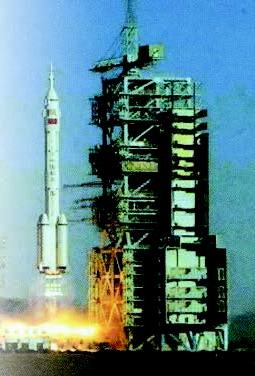
\includegraphics[height=9.0cm]{8-9.jpg}
    \caption{}\label{fig:8-9}
  \end{minipage}
  \begin{minipage}[b]{0.48\linewidth}\centering
    \includegraphics{8-10.pdf}
    \caption{多级火箭}\label{fig:8-10}
  \end{minipage}
\end{figure}

理论计算表明,火箭获得的最终速度主要取决于两个条件,一个是喷气速度,一个是质量比,即火箭开始飞行时的质量与燃料燃尽时的质量之比。
为了提高喷气速度,需要使用高质量的燃料,目前常用的液体燃料是液氢,用液氧做氧化剂。
质量比与火箭的结构和材料有关系,现代技术能达到的质量比不超过 10。
在现代技术条件下,用一级火箭还不能达到发射人造卫星所需要的速度。
要发射人造卫星,现在都用多级火箭。

多级火箭是由单级火箭组成的(\cref{fig:8-10})。
发射时先点燃第一级火箭,它的燃料用完以后空壳就自动脱离。
这时第二级火箭开始工作,第二级火箭在燃料用完以后空壳也自动脱离,以后又是下一级火箭开始工作。
多级火箭在工作中及时把对后面航行没有用的空壳抛掉,使火箭的总质量减少,因此能够达到很高的速度,可以用来发射人造卫星、宇宙飞船和洲际导弹。
当然,火箭的级数也不是越多越好,因为级数越多,火箭的构造也越复杂,工作的可靠性也越差。
目前,多级火箭一般都是三级的。

现代的火箭,工作时推力的大小很不一样。
小的如空对空导弹的火箭,推力只有几万牛,大的如发射人造卫星的火箭和洲际导弹的火箭,推力可达几百万牛以上。

火箭技术与科学技术和国防的现代化都有很大的关系,是现代的一门重要尖端技术。
我国已经运用自己研制的火箭多次发射过人造卫星和远程导弹。
我们还要进一步提高火箭技术,尽快地赶上和超过国外的先进水平。
我们相信,在同学们中,一定会有人在这一重要领域内为祖国作出卓越的贡献!

\begin{Review}
\begin{question}
  \item 什么是冲量?什么是动量?冲量一定时,作用力的大小与力的作用时间有什么关系?动量一定时,物体的质量与运。动速度之间有什么关系?
  \item 什么是动量定理?
  \item 什么是动量守恒定律?
  \item 什么叫弹性碰撞?什么叫非弹性碰撞?什么叫完全非弹性碰撞?哪种碰撞动能的损失最大?
\end{question}
\end{Review}

\begin{Exercise}*
\begin{question}
  \item 质量为 \qty{1}{kg} 的手榴弹以 \ang{60} 角斜抛出去,抛出的速度为 \qty{10}{m/s},手榴弹到达最高点时炸成两块,一块的质量是 \qty{0.6}{kg},以 \qty{15}{m/s} 的速度沿原方向运动,求另一块的速度大小和方向。
  \item 对于在一直线上运动的两个物体组成的系统,动量守恒定律的一般表达式为:
\[m_1v_1+m_2v_2=m_1v'_1+m_2v'_2.\]
  在不同情况下,这个表达式往往可以简化为不同形式,试写出下列各种情况下得出的简化的表达式:
\begin{enumerate}
  \item 两个物体原来静止,发生相互作用后分开;
  \item 一个物体原来静止,另一个物体跟它碰撞后粘合在一起并共同沿原来的方向运动;
  \item 一个物体原来静止,另一个运动物体与它正碰后,两物体以不同的速度在原来的直线上运动;
  \item 两个相向运动的物体,相碰后都静止下来。
\end{enumerate}
  \item 试证明:两个物体碰撞后,它们的速度变化 $\Delta v_1=v'_1-v_1$ 和 $\Delta v_2=v'_2-v_2$ 跟它们的质量成反比,即
  \[\frac{\Delta v_1}{\Delta v_2}=-\frac{m_2}{m_1}\]
  并利用所得结果来讨论:很轻的物体(如乒兵球)跟一个很重的物体(如课桌)碰撞后,它们的速度变化有什么特征。
  \item 质子的质量是\qty{1.67e-27}{kg},速度为 \qty{1e7}{m/s},与一个静止的氦核碰撞后,质子以 \qty{6e6}{m/s} 的速度反弹回来,氦核以 \qty{4e6}{m/s} 的速度向前运动。
  \begin{enumerate}
    \item 你能否求出氦核的质量?如果能,是多少?
    \item 你能否求出碰撞时的相互作用力?为什么?
  \end{enumerate}
  \item 两个球以相同的速度相向运动,其中一个球的质量是另一个的三倍,相碰后重球停止不动,轻球以二倍的速率弹回,试证明它们发生的是弹性碰撞。
   \item 在光滑水平面上一个质量为 \qty{0.2}{kg} 的小球以 \qty{5}{m/s} 的速度向前运动,途中与另一个质量为 \qty{0.3}{kg} 静止的小球发生正碰。假设碰撞后第二个小球的速度为 \qty{4.2}{m/s},你算出的第一个小球的速度是多大?想一想,这种情况真的可能发生吗?这道题的毛病出在哪里?
\begin{figurehere}
  \begin{minipage}{\linewidth}\centering
    \includegraphics{8-11.pdf}
    \caption{}\label{fig:8-11}
  \end{minipage}
\end{figurehere}
  \item 一个质量 $M=\qty{0.2}{kg}$ 的小球放在高度 $h=\qty{5}{m}$ 的直杆顶端(\cref{fig:8-11}),一颗质量 $m=\qty{0.01}{kg}$ 的子弹以 $v_0=\qty{500}{m/s}$ 的速度沿水平方向击中小球,并穿过球心,小球落地处离杆的距离 $s=\qty{20}{m}$。求子弹落地处离杆的距离。子弹的动能有多少转化成了热能?
   \item 一个连同装备共有 \qty{100}{kg} 的宇宙航行员,脱离宇宙飞船后,在离飞船 \qty{45}{m} 处与飞船处于相对静止状态。他带着一个装有 \qty{0.5}{kg} 氧气的贮氧筒,贮氧筒有个可以使氧气以 \qty{50}{m/s} 的速度喷出的喷嘴,宇航员必须向着与返回飞船相反的方向释放氧气,才能回到飞船上去,同时又必须保留一部分氧气供他在飞回飞船的途中呼吸。飞行员呼吸的耗氧率为 \qty{2.5e-4}{kg/s}。如果他在开始返回的瞬间释放 \qty{0.1}{kg} 的氧气,他能安全回到飞船吗?

% \begin{solution}
%     宇航员向着与返回飞船相反的方向释放出$m=0.1$
% 千克的氧气后,他将获得向着飞船运动的速度。要知道宇航员能否安全回到飞船,先要求出它返回飞船需要的时间$t$。取飞船为参照物,向着飞船运动的方向为正方向,氧气释放的速度$v=-50\ms$。设宇航员获得的速度为$V$,宇航员连同装备的总质量为$M$。原来宇航员相对于飞船是静止的,根据动量守恒定律可得:
% \[(M-m)V+mv=0\]
% 考虑到$M\gg m$,得$MV+mv=0$,所以
% \[V=-\frac{mv}{M}\]
% 设宇航员离飞船的距离为$d$,他返回飞船所需的时间
% \[t=\frac{d}{V}=-\frac{Md}{mv}=-\frac{100\times 45}{0.1\times (-50)}=900{\rm s}\]

% 宇航员呼吸的耗氧率$R=2.5\times 10^{-4}{\rm kg}/{\rm s}$,在返回飞船这段时间$t$内他呼吸需要的氧气
% \[m=Rt=2.5\times 10^{-4}\times 900{\rm kg}=0.23{\rm kg}\]

% 他释放0.1千克的氧气后,筒内剩余的氧气是
% \[ m_{\text{余}}=0.5-0.1=0.4{\rm kg}\]

% 由于他剩余的氧气多于他返回途中呼吸所需的氧气,因
% 此他可以安全返回飞船。
% \end{solution}

\item 在上题中,如果宇航员想以最短的时间返回飞船,他开始最多能释放出多少氧气?这时他返回飞船所用的时间是多少?
\item 速度为\qty{e5}{cm/s} 的氦核与静止的质子发生正碰,氦核的质量是质子的 4 倍,碰撞是弹性的,求碰撞后两个粒子的速度。
\item 一个质量是 $m_1$,动能是 $E_K$ 的物体与一个质量是 $m_2$ 的不动的物体正碰,假定发生的是弹性碰撞,在 $m_1=0.01m_2$,$m_1=m_2$,$m_1=100m_2$ 的情况下,$m_1$ 传递给 $m_2$ 的动能各是多少?(有兴趣的同学还可以进一步讨论 $m_1$ 传递给 $m_2$ 的动能最大或最小的条件)。

  \item 在有些原子反应堆里,要让中子与原子核碰撞,以便把中子的速率迅速降低下来。为此,是选用较重的还是较轻的原子核效果较好?为什么?
\end{question}
\end{Exercise}